\chapter{Juegos serios}
\label{chap:juegos_serios}


Un juego serio es un vídeojuego elaborado con el propósito primario que no es el
de entretener\cite{sg:aoverview}, sino tiene una finalidad educativa explícita y
cuidadosamente pensada, utiliza la tecnología y los conceptos de la industria de
los vídeojuegos para encontrar solución a problemas reales. Es una corriente que
se utilizan para definir los juegos que poseen una pedagogía incluida, algún
tipo de evaluación ya sea interna o externa y lo que hay que aprender
(contenido) integrado\cite{damien:sg}.

A continuación se describen las principales características de un juego serio, y
diferentes corrientes que evolucionan de manera paralela, compartiendo conceptos
y apoyándose mutuamente.

Se presenta un modelo de desarrollo que fue utilizado en el desarrollo de un
juego serio denominado \textit{Living Forest}, y a continuación se describe la
actualidad de los juegos serios, incluyendo las conferencias más importantes y
casos de éxito actuales.

Por simplicidad, se utiliza el término juego para referirse a un videojuego, así
juegos serios se refiere a videojuegos serios.

\section{Características}

Los \emph{Serious Game} proveen una oportunidad muy importante para ayudar en la
enseñanza y desarrollo de profesionales, por que ayudan a crear el tipo de
educación que los adultos prefieren, proveen mecanismos para que los estudiantes
cometan errores y experimenten con sus ideas, con su conocimiento y con la
teoría en un ambiente protegido sin riesgos para la vida o la identidad. 

Los beneficios que brindan los \emph{Serious Game} se acentúan en la medida en
la que los mismos proveen entornos más completos en donde realmente se puedan
poner en práctica la teoría, esto ayuda a una comprensión más profunda del área
de interés.

La principal diferencia entre los \emph{Serious Game} y otras aplicaciones de
\emph{E-Learing} es su enfoque en la creación de una experiencia de aprendizaje
significativo, relevante y atractivo. En un \emph{Serious Game} existen metas
claras de aprendizaje pero las mismas se encuentran en un contexto significativo
en donde se deben aplicar los conocimientos y hacer uso de herramientas que
están a disposición para obtener éxito en la resolución de los problemas
presentados. Estos problemas se equilibran a través de la retroalimentación y
otras estrategias para mantener el interés del estudiante\cite{papertian:const}.

El campo de los \emph{Serious Game} rechaza la idea de que los profesionales de
la educación pueden ser reemplazados fácilmente, para ellos la labor de estos
profesionales es imprescindible para la reflexión y orientación del aprendizaje.
Es cierto que se puede llegar a aprender sin el apoyo de un profesional de la
educación pero se corre el riesgo de perder el enfoque y la eficacia
\cite{elearning:seiousgames}. 

El \emph{serious Game} no se trata de una modelo de aprendizaje pasajero. Varios
autores como \emph{Johan Huizinga}, \emph{Jean Piaget}, \emph{Wittgenstin} y
\emph{Seymour Papert} han reconocido su importancia como objeto de aprendizaje.
Los juegos deben ser elaborados teniendo en cuenta el nivel cognitivo del
estudiante, es decir, su etapa de aprendizaje y en que el aprendizaje difiere de
acuerdo a la etapa de vida en la que se encuentre un estudiante. Mediante la
práctica repetida de actividades relacionadas al área de interés se desarrollan
habilidades y destrezas\cite{education:games}.

\subsection{Ventajas}


Las \Gls{tic} y los juegos serios en particular son herramientas de inestimable
valor para apoyar los nuevos procesos de enseñanza-aprendizaje y
evaluación\cite{guenaga2013serious}.

Los juegos serios, constituyen un escenario privilegiado para el desarrollo de
todos los componentes de las competencias (conceptos, habilidades, actitudes,
motivaciones, valores, etc.) ya que permiten desarrollar vivencias en las que
ponerlos en práctica, permitiendo el entrenamiento en situaciones que en muchas
ocasiones son similares a las que se encuentran en entornos
reales\cite{guenaga2013serious}.

Además, favorecen la autoestima y tienen un factor motivacional, así como la
posibilidad de desarrollar destrezas y estrategias cognitivas como la capacidad
de resolución de problemas, toma de decisiones, búsqueda y organización de la
información, habilidades perceptivo-motrices y razonamiento
abstracto\cite{guenaga2013serious}.

Se puede añadir también que aumentan la capacidad de coordinación, percepción
espacial y ampliación del campo visual, lo que tiene una incidencia en la
lectura y el manejo eficiente en ambientes 3D\cite{guenaga2013serious}. 

Más allá del logro de competencias puntuales, las teorías modernas de
aprendizaje sugieren que el aprendizaje es más efectivo cuando es activo,
experiencial, situado, basado en problemas y se recibe retroalimentación
inmediata y los juegos basado en aprendizaje se fundamentan en esos
principios\cite{guenaga2013serious}.



\subsection{Desafíos}


El potencial de un juego serio no es ilimitado, los desarrolladores se
encuentran con múltiples desafíos que deben ser superados para poder obtener un
juego serio que obtenga las ventajas citadas previamente y pueda ser de utilidad
en la educación formal.

Un juego serio, como el resto de la \textit{media}, no puede cambiar el
comportamiento de una persona por sí solo, un juego acerca de hábitos
saludables, no hará del jugador un nutricionista, pero si permiten al jugador
explorar las opciones, tener en cuenta las consecuencias de sus actos y poner en
práctica su conocimiento\cite{education:games}, adicionalmente es importante
definir lo que forma parte del juego serio y lo que no, pues un juego serio no
debe incluir todas las características de la
realidad\cite{stapleton2004serious,videojuegos:gonzaleztardon}. 

La forma tradicional de evaluación presenta dificultades a los juegos serios,
por ejemplo, las pruebas tradicionales contienen un grupo de preguntas, las
cuales son vistas de manera independiente, en cambio en un juego serio, las
acciones son dependientes del contexto y las acciones previamente
realizadas\cite{shute2009melding}.

En cuanto al objeto pedagógico, el área en la cual se utiliza un juego serio es
un factor determinante para el éxito del mismo, es decir, se debe responder a la
pregunta: \emph{¿Es necesaria una solución basada en juegos
    serios?}\cite{stapleton2004serious}, las áreas de aplicación de un juego
serio se describen con más detalle en~\ref{sec:areas_aplicacion}.

Uno de los factores más complicados a la hora del desarrollo de juegos serios es
la limitación de recursos financieros, esto no quiere decir que no existan
recursos para su desarrollo, sino que, comparados con los recursos invertidos en
otras \textit{media} es insignificante\cite{stapleton2004serious}. Como
consecuencia de las limitaciones financieras, los desarrolladores no siempre
pueden acceder a tecnología de última generación\cite{stapleton2004serious}

\section{Corrientes relacionadas}

Los juegos serios son el solapamiento de tres corrientes, los videojuegos, las
técnicas de enseñanza y la simulación educativa\cite{education:games}, tal y
como se observa en la figura~\ref{fig:corrientes_relacionadas}. 

\begin{figure}[ht]
\centering
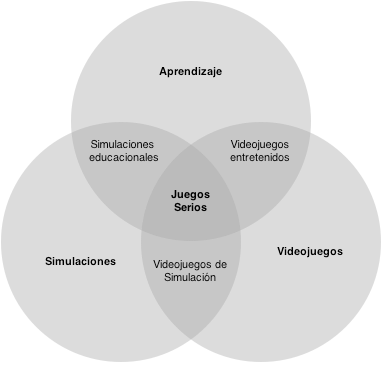
\includegraphics[scale=0.7]{juegos_serios/corrientes_paralelas.png}
\caption{Ubicación de los juegos serios entre los videojuegos, la simulación y
    la educación}
\label{fig:corrientes_relacionadas}
\end{figure}

Cuando se utilizan aspectos de videojuegos con simulaciones, se obtienen videojuegos,
cuyo objetivo es entretener mientras son similares a la realidad, dentro de esta
categoría podemos encontrar juegos como \emph{Gran Turismo}; sí mezclamos
factores relacionados al aprendizaje y a las simulaciones se obtienen
simulaciones sin interacción con el usuario que buscan mostrar o enseñar como se
comportan distintos fenómenos físicos, sociales, etc.

Los \emph{Edutainment} pueden ser vistos como los predecesores de los juegos
serios, los mismos son descritos en~\ref{sec:edutainment}.

\subsection{Simulaciones educativas}


La simulación se define como el proceso de diseñar un modelo de un sistema real
y, llevar a cabo experimentos con este modelo, con el fin o bien de entender el
comportamiento del sistema o de la evaluación de distintas estrategias para la
operación del sistema\cite{ingalls2008introduction}. 

Aunque un juego serio y una simulación pueden parecer muy similares, se
diferencian en que, si bien muchos videojuegos incluyen una simulación, una
simulación no utiliza características típicas de los videojuegos como la fantasía,
puntuación, etc\cite{sg:aoverview}.

La simulación en el ámbito de la educación evolucionó desde simples motores de
reglas hasta complejos entornos. La simulación demostró ser una herramienta muy
útil en el ámbito laboral\cite{mariluz:seiousgames}, pues enseña al usuario a
encarar situaciones muy difíciles de representar en entornos completamente
controlados y provee mecanismos para comprobar la efectividad de la herramienta. 

Actualmente la simulación se utiliza más en el ámbito empresarial pues las
empresas son las más necesitadas de innovar en el ámbito de la enseñanza. Un
ejemplo de esta necesidad se da, por ejemplo, en el entrenamiento de nuevos
vendedores, es muy difícil enseñar a un vendedor como debe vender los productos
con un pizarrón y/o una presentación, en cambio la simulación permite que el
mismo pueda probar cosas nuevas y experiencias de sus compañeros (o instructor),
convirtiendo así el aprendizaje en colectivo\cite{mariluz:seiousgames}.

Existen dos tipos de simulaciones, en primer lugar están las experimentales que
ponen al estudiante en el lugar de un profesional y requieren que el mismo tome
decisiones para alcanzar los objetivos y en segundo lugar están las simbólicas
que buscan que el estudiante deduzca eventos, principios y mejores
prácticas\cite{charsky:2010}. 


\subsection{Diferencia entre juegos serios, simulaciones y los Edutainment}

Estos tres entornos virtuales altamente interactivos, poseen posibilidades y
fines distintos, pueden parecer similares pero poseen las siguientes
diferencias\cite{education:games}:

\begin{itemize}
\item \textbf{Simulaciones educativas}: utilizan escenarios rigurosamente
    estructurados con un conjunto altamente refinado de normas, retos y
    estrategias que son cuidadosamente diseñados para desarrollar las
    competencias específicas que se pueden transferir directamente al mundo
    real.
\item \textbf{Videojuegos:} son actividades atractivas y divertidas que
    habitualmente se utilizan exclusivamente para el entrenamiento pero también
    permiten una exposición con un conjunto determinado de herramientas,
    argumentos o ideas. Todas las partidas se juegan en un mundo estructurado
    por normas específicas, mecanismos de retroalimentación, y las herramientas
    necesarias, aunque no están tan definidas como en las simulaciones.
\item \textbf{Edutainment:} son aplicaciones educativas cuyo principal propósito
    es el de entretener, y el aprendizajes es un añadido. Los
    \emph{edutainment}, se centran en la motivación externa.
\end{itemize}

\section{Desarrollo de juegos serios}
\label{sec:desarrollo}

Una vez definido lo que es un juego serio, queda la tarea de definir cómo
realizar uno, incluyendo qué factores deben ser tomados en cuenta durante su desarrollo.
% Esto hacemos/ esto de los problema comunes? wtf no me acuerdo de haber leido nunca esto

Según~\cite{education:games} un juego serio debe cumplir los siguientes
tres criterios:

\begin{itemize}

\item \textbf{Implementación técnica}: se refiere a la actividad de programación
    y ejecución de un patrón de diseño. Incluye la perfecta integración de los
    elementos de diseño en el videojuego. 

\item \textbf{Adecuación para la educación:} la capacidad del videojuego para hacer
    frente a las metas curriculares o educativas y la habilidad o el
    conocimiento del jugador relativo a los contenidos educativos que se aborde.

\item \textbf{Integración total con los objetivos pedagógicos:} la integración
    del patrón de diseño y el videojuego en general con los objetivos
    educativos.

\end{itemize}


Adicionalmente, el diseño del mismo se tiene que centrar en cuatro factores o
dimensiones, las cuales son\cite{education:games}:

\begin{itemize}
\item \textbf{Contexto:} es decir, donde ocurre el aprendizaje, lo que va desde
    aspectos macro, como  factores políticos, económicos e históricos, hasta
    aspectos micro como la experiencia y  antecedentes de los profesores, costos
    de licencia, entre otros.
\item \textbf{Tipo de aprendizaje:} para el individuo o grupo, requiere que se
    considere su  estilo de aprendizaje y sus conocimientos previos, y qué
    métodos se ajustan mejor a sus  necesidades.
\item \textbf{Modo de representación:} lo que incluye el nivel de interactividad
    requerido, la fidelidad y  el nivel de inmersión producido. Además cubre la
    narración de los hechos, la separación de los  aspectos de inmersión con la
    reflexión de haber utilizado el videojuego. Y de manera importante  enfatiza
    el potencial de retroalimentación que refuerza el aprendizaje.
\item \textbf{Principios pedagógicos:} es necesario reflexionar sobre los
    modelos de aprendizaje lo  que permite producir apropiados planes de
    lecciones.
\end{itemize}

Estas dimensiones no pueden ser consideradas individualmente, todas están
relacionadas  como se muestra en el figura~\ref{fig:desarrollo_dimensiones}.

\begin{figure}[H]
\centering
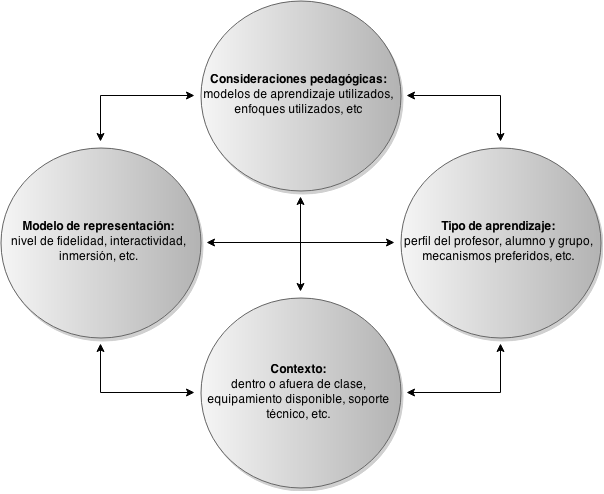
\includegraphics[scale=0.5]{juegos_serios/desarrollo_dimensiones.png}
\caption{Relación entre las cuatro dimensiones a considerarse en un videojuego
    basado en aprendizaje}
\label{fig:desarrollo_dimensiones}
\end{figure}

A continuación se da un ejemplo de flujo de diseño para implementar un juego serio 
manteniendo todas sus características incluyendo los criterios y factores descritos 
anteriormente.

\subsection{Flujo de diseño de un juego serio}

\textit{Pereira}\cite{pereira2009design} en el diseño del videojuego \emph{Living
    Forest} utiliza un conjunto de pasos bien definidos como modelo de creación
de un juego serio a partir de la definición previa de las competencias básicas
que se desean enseñar.

Es importante notar que este modelo se adecua a las dimensiones y criterios
definidos previamente. La obtención de las competencias básicas no forma parte
de este flujo pues, se asume que es un paso previo al diseño.

\begin{figure}[ht!]
\centering
\begin{tikzpicture}[auto]
    % Place nodes
    \node [block] (1) {1. Objetivos de diseño};
    \node [block, right of=1, node distance=5cm] (2) {2. Competencias básicas relacionadas con la educación};
    \node [block, right of=2, node distance=5cm] (3) {3. Investigación del dominio};
    \node [block, below of=3, node distance=3cm] (4) {4. Diseño del juego};
    \node [block, left of=4, node distance=5cm] (5) {5. Tiempo en el juego};
    \node [block, left of=5, node distance=5cm] (6) {6. Acciones de jugabilidad};
    \node [block, below of=6, node distance=3cm] (7) {7. Indicadores};
    \node [block, right of=7, node distance=5cm] (8) {8. Representación e interacción};
    \node [block, right of=8, node distance=5cm] (9) {9. Implementación};
    \node [block, below of=9, node distance=3cm] (10) {10. Evaluación};
    % Draw edges
    \path [line] (1) -- (2);
    \path [line] (2) -- (3);
    \path [line] (3) -- (4);
    \path [line] (4) -- (5);
    \path [line] (5) -- (6);
    \path [line] (6) -- (7);
    \path [line] (7) -- (8);
    \path [line] (8) -- (9);
    \path [line] (9) -- (10);
\end{tikzpicture}
\caption{Flujo de diseño propuesto de un juego serio}
\label{fig:tics_flujo_diseño_prop}
\end{figure}

Teniendo las competencias básicas que se desea sean enseñadas, practicadas o
perfeccionadas por el usuario mientras utiliza el juego serio a diseñar, los
siguientes puntos que deben ser diseñados son
(ver~\ref{fig:tics_flujo_diseño_prop}):

\begin{enumerate}
\item \textbf{Objetivos de diseño:} definen cuál es el propósito del videojuego, donde
    se toman en cuenta los objetivos pedagógicos, así como también objetivos que
    garanticen que el mismo sea agradable, intuitivo y motivador.

\item \textbf{Competencias básicas relacionadas con la educación:} se identifican
    aquellas que influyen en el diseño del videojuego, se definen los conocimientos
    mínimos que se desea que tenga un usuario que lo utilice.

Las competencias básicas pueden tener diferentes orígenes, en el ámbito
académico se puede utilizar el plan de estudios, en una empresa se pueden
utilizar los objetivos y la visión de la misma.

\item \textbf{Investigación del dominio:} esta fase se encarga de recabar
    información exacta acerca del dominio en el cual se desenvuelve el juego
    serio, en esta fase es importante que participe un experto en el dominio,
    por ejemplo, en el ámbito académico se puede contar con un profesor experto
    en el dominio.

Es importante realizar la pregunta \emph{¿Qué nivel de detalle es necesario?},
para así definir qué contenido incluir, y qué factores se deben analizar.

Además es necesario investigar las acciones que se podrían realizar dentro del
videojuego, cómo se desenvolverá el jugador, por cada acción definida, se deben
analizar los elementos y factores relacionados que se deben modelar.

\item \textbf{Diseño del juego:} a partir de la idea original y basado en la
    información recogida se determina el papel desempeñado por el jugador (de
    acuerdo a la semántica y pragmática de las acciones y decisiones que está
    llamado a hacer). 

Se define el nivel de aproximación a la realidad, el nivel de detalle del
entorno, del jugador y de las acciones.

Otro factor que se debe tener en cuenta en esta fase es la cantidad de tiempo
que pasará un jugador en el juego, se deben modelar todas las acciones del
jugador y el entorno de acuerdo a este tiempo.

\item \textbf{Tiempo de juego:} el primer factor que se debe estudiar es el
    período de adaptación del jugador, lo que depende de la intuitividad del
    videojuego, este tiempo debe ser analizado por separado a la hora de realizar un
    análisis de los resultados.
    
    Se debe definir la duración de las partidas y la forma en la que 
    se mostrarán los resultados de las acciones.
% Esto es jodido por que no hicimos, osea mmm no se
%Si el videojuego tiene una duración reducida, se tienen que analizar mecanismos %para
%mostrar los resultados de las decisiones a largo plazo, además de como mostrar
%los resultados de las acciones de corto plazo.

\item \textbf{Indicadores:} es todo aquello que muestre información relevante al
    jugador acerca de su estado, ejemplos de este tipo de indicadores son el
    puntaje, tiempo empleado, objetivos cumplidos. 

La definición de como se juzgará la calidad de una partida del jugador debe ser
definida, normalmente mediante un puntaje general, el mismo debe mostrar
claramente los resultados de las acciones, si las mismas fueron positivas o
negativas para el logro final de los objetivos.

\item \textbf{Representación e interacción:} representación se refiere a como se
    visualiza el entorno, e interacción a como se relaciona el jugador con su
    entorno.

Se inicia con un bosquejo de las representaciones de la escena del videojuego, para
así poder definir los elementos que forman parte de la escena.

Otros bosquejos necesarios son los del concepto que se modela en la lógica del
videojuego, para así definir las animaciones del entorno y del jugador.

Se deben definir las alertas sonaras, qué partes del entorno produce sonidos,
cómo el jugador recibe estas alertas (por ejemplo si el origen de las mismas es
siempre el mismo o importa la distancia a la cámara), se puede agregar música de
ambiente si el videojuego lo amerita.

Se define la interfaz del usuario, qué información será representada, las
acciones disponibles desde la misma, además se define si el mismo será en
primera persona (la cámara son los ojos del jugador) o en tercera persona (la
cámara se sitúa inmediatamente atrás y arriba de la cabeza), como será la
interacción con la cámara, acercamientos y movimientos para contemplar el
entorno.

\item \textbf{Implementación:} en esta etapa se estudia el estado del arte de las
    plataformas tecnológicas disponibles para el desarrollo del videojuego, se toman
    en cuenta los factores como la disponibilidad de componentes, de
    documentación, lenguajes de programación y herramientas de pruebas
    automáticas.

El proceso puede ser iterativo, entre sesiones de implementación y evaluación de
lo implementado, para así poder realizar optimizaciones enfocadas especialmente
en la estética, la retroalimentación y el estado del jugador.

\item \textbf{Evaluación:} durante el desarrollo del juego serio, se deben
    realizar varias sesiones de evaluación, por ejemplo, con los responsables o
    expertos y miembros de la audiencia objetivo. Así mismo, se deben realizar
    evaluaciones con los grupos de interés las cuales se centran en la adaptación
    del videojuego (usabilidad). 

La primera evaluación mencionada se centra en la validación del modelo de la simulación
(refinamiento), mientras que la segunda evaluación sirve para probar el videojuego en
un escenario (parecido al final) y evaluar los aspectos relacionados con el
proceso de aprendizaje.  

\end{enumerate}

\section[Ejemplos]{Ejemplos de juegos serios}

En este apartado se darán detalles de varios casos de éxito de aplicaciones que
tienen como objetivo ayudar en el aprendizaje del usuario o jugador en algún
tema en particular.

Se presentan varios casos de éxito, donde se puede ver cómo la utilización de
las \Gls{tic} provocaron un resultado positivo en las personas que lo
utilizaron.

\subsubsection{Triage Trainer}

\begin{itemize}
\item \textbf{Tipo:} Simulación de entrenamiento.
\item \textbf{Destinatarios:} Médicos, enfermeros, paramédicos y otros
    rescatistas.
\item \textbf{Contenido:} Entrenamiento para evaluar a los pacientes en un lugar de
  emergencia.
\item \textbf{Desarrollador:} \emph{TruSim}.
\end{itemize}

\begin{figure}[ht!] 
\centering 
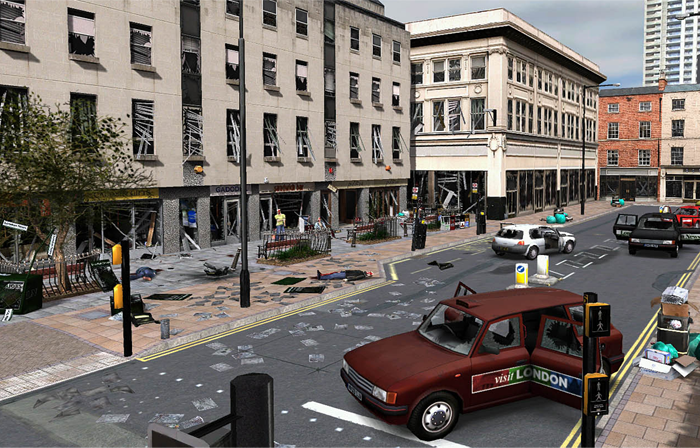
\includegraphics[scale=0.5]{tics/images/triage.png}
\caption{Ambientación de Triage}
\label{fig:triage}
\end{figure}

\emph{Triage Trainer} se desarrolla \fixme{en una escena de explosión}{Refinar,
    decir algo más intermedio, y no empezar por detalles} en una calle
(ver~\ref{fig:triage}) la cual es un incidente mayor, y está diseñado para
formar profesionales que puedan participar en una escena de un incidente de este
tipo (médicos, enfermeros, paramédicos, rescatistas). Los jugadores deben
realizar un triage, es decir, evaluar el grado de las lesiones de víctima, las
cuales son generadas aleatoriamente, utilizando los protocolos y controles
médicos adecuados, además de priorizar a las víctimas para el tratamiento. La
apariencia física de cada víctima es imitada con precisión como los signos
vitales, los síntomas y sobre todo los patrones de tiempo para el deterioro de
las lesiones, es decir, la condición de una víctima cambia de forma realista con
el tiempo (ver~\ref{fig:triage_patient1}).

\begin{figure}[ht!]
\centering 

\includegraphics[scale=0.5]{tics/images/patient_side.jpg}
\caption{Evolución de un paciente en Triage}
\label{fig:triage_patient1}
\end{figure}

Al finalizar cada simulación los jugadores reciben retroalimentación acerca de
su rendimiento, incluyendo la precisión de sus chequeos, si los pacientes fueron
priorizados en el orden correcto y el tiempo que les llevó completar el triage,
en comparación con la de un experto.

La retroalimentación de los participantes que utilizaron Triage Trainer sugiere
que el mismo cumplió exitosamente sus fines. Los jugadores asociaron su
experiencia en el videojuego con su experiencia en el mundo real y muchos de ellos
sentían que realmente estaban allí. Se espera que los jugadores puedan tomar
decisiones bajo presión, lo que ayudará a su desarrollo cognitivo. También se
observó que los jugadores tienden a discutir sus experiencias con sus compañeros
de curso, lo que también podría tener un impacto en su aprendizaje.

Un elemento que no fue evaluado por \emph{TruSim} debido a que no era
logísticamente posible fue el impacto de las pruebas en la retención del
conocimiento y el cambio de comportamiento de los
jugadores\cite{education:games}. 


\subsubsection{SimVenture}

\begin{itemize}
\item \textbf{Tipo:} Juego de simulación de negocios.
\item \textbf{Destinatarios:} Personas de 14 a 30 años.
\item \textbf{Contenido:} Las realidades de la creación y funcionamiento de un
    negocio.
\item \textbf{Desarrollador:} \emph{Venture Simulations.}
\end{itemize}

En el inicio del videojuego (ver~\ref{fig:simventure_tutorial}), a los jugadores se
les brinda informaciones y antecedentes para que que se ubiquen en escena. Ellos
deben empezar a dirigir su propio negocio en su casa de fabricación y venta de
computadoras, mientras deben mantener un trabajo de tiempo completo
independiente. El videojuego lleva a los jugadores a la ejecución de un negocio en su
propia casa y a la extensión del mismo a más locales, lo que requiere
contratación de personal. Los jugadores son capaces de avanzar en el videojuego a
través del aprendizaje de los elementos importantes de la empresa, organizadas
en cuatro categorías: organización, ventas/marketing, finanzas y operaciones.
Los jugadores toman decisiones acerca de las actividades dentro de estas áreas y
observan los resultados de sus acciones. 

\begin{figure}[ht!]
\centering 
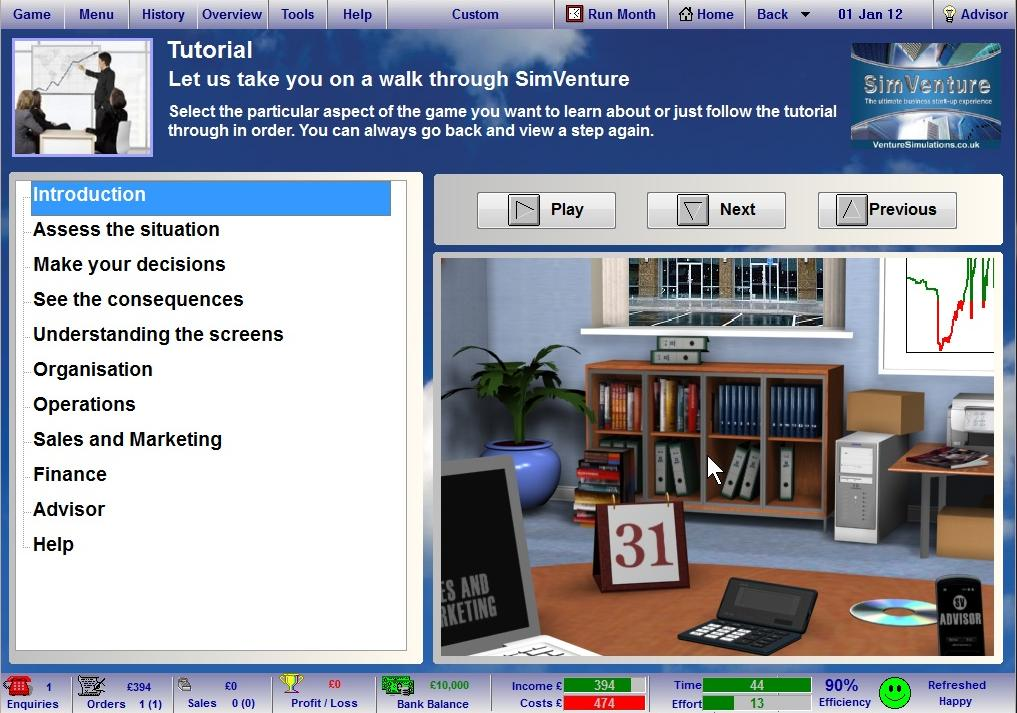
\includegraphics[scale=0.5]{tics/images/simventure-tutorial.jpg}
\caption{Tutorial de SimVenture}
\label{fig:simventure_tutorial}
\end{figure}

Los jugadores obtienen retroalimentación sobre un número de diferentes
parámetros. En un nivel básico, se puede simplemente revisar la cantidad de
ingresos que están generando. Además de esto, el éxito puede ser medido por la
cantidad de pedidos que han recibido para sus productos. También se proporciona
retroalimentación visual para representar la eficiencia de la organización y su
felicidad como individuo.

\emph{Phil Warren}, director de estudios de negocios en \emph{Snaith School}, ha
utilizado \emph{SimVenture} como complemento al plan de estudios. Según el
mismo, el plan de estudios por lo general sólo requiere que los estudiantes
aprendan sobre los diversos elementos del negocio de forma aislada, sin embargo
en la realidad, cualquier decisión que se tome en una de las partes de un
negocio tiene efecto en las demás. \emph{SimVenture} se vio como una oportunidad
de aplicar los conocimientos aprendidos en clase en una actividad práctica,
además se observó que permitir que los estudiantes jueguen en pares da un
espacio para la discusión en torno a las decisiones y aprenden de sus errores
juntos\cite{education:games}.

\section{Actualidad}

La relación de los videojuegos con el aprendizaje surge en los años $80$ y ha llegado
hasta la actualidad en plena efervescencia, siendo aplicados en casi todos los
ámbitos de la educación tanto formal como no formal. Los juegos serios para el
entrenamiento de habilidades se pueden considerar una evolución de las técnicas
de entrenamiento basadas en la realidad virtual que se desarrollaron en los años
$90$ y que en la actualidad se han transformado, por su potencial motivacional,
de simulaciones puras a juegos\cite{videojuegos:gonzaleztardon}.

Al ser un área de creciente interés, existe una gran cantidad de conferencias
cuyo objetivo es el estudio de los juegos serios en la educación, se presenta un
resumen de algunas de ellas:

\begin{itemize}
\item \textbf{Games beyond Entertainment Week}: es una serie de conferencias
    cuyo objetivo es explorar los juegos serios, sus oportunidades de mercado,
    se centra en redes, promoción, desarrollo comercial. Una de sus
    conferencias, es la \emph{Games for health}, la cual se enfoca
    específicamente en el cuidado de la salud, agrupa a profesionales de la
    salud y de los juegos serios\cite{games_beyond_entertainment}.
\item \textbf{Serious games Development and Applications}: es una conferencia
    que se desarrolla desde el $2010$, apunta a coleccionar y distribuir todo el
    conocimiento relacionado a los juegos serios, para así proveer un foro de
    discusión sobre la actualidad del desarrollo de los juegos
    serios\cite{sgda}.
\item \textbf{Gaming and Learning Conference}: es una conferencia dedicada al
    estudio y aplicación de los juegos serios, incluye una presentación donde
    los desarrolladores pueden mostrar sus productos. Se interesa además en
    potenciales inversores para el desarrollo de videojuegos, así como a
    desarrolladores, investigadores y jugadores\cite{gala}.
\item \textbf{Serious Play Conference}: es una conferencia dedicada a expertos
    con poder de decisión sobre organizaciones gubernamentales, el foco
    principal de la conferencia es explorar las oportunidades, desafíos y
    potencial de juegos serios desarrollados por los
    participantes\cite{seriousplay}.
\end{itemize}

Existen otras conferencias que no se centran exclusivamente en los juegos
serios, pero que por su naturaleza incluyen presentaciones sobre el tema, por
ejemplo, la \emph{DiGRA} (\textit{Digital Games Research Association}), se
centra en el desarrollo y la investigación de los videojuegos en general, pero
se han presentado numerosos artículos relacionados a  los juegos serios; la
\emph{Vs-Games}, que trata sobre entornos virtuales y videojuegos con  aplicaciones
más allá del entretenimiento.

Estas conferencias abarcan diferentes áreas o ámbitos de aplicación de los
juegos serios, que van desde lo militar hasta el cuidado de la salud.

\subsection{Áreas de aplicación}
\label{sec:areas_aplicacion}
\observacion{Revisar si no conviene mover esto mas adelante}

A continuación se definen las áreas de utilización  más frecuentes de juegos serios, son en 
estas áreas donde los juegos serios demuestran su fortalezas,

\begin{itemize}

\item \textbf{Militar}: Los primeros videojuegos a menudo \fixme{se basaban}{}
    en lucha o combate. Durante más de $30$ años los videojuegos han sido
    reconocidos como herramientas factibles en el entrenamiento de militares. En
    $1996$ fue lanzado un videojuego llamado \emph{Marine Doom} en donde la
    tarea de los jugadores era el aprendizaje de formas de ataque, conservación
    de municiones, comunicarse con eficacia, dar órdenes al equipo de trabajo
    entre otros. De esta manera tuvo lugar una forma de entrenamiento más
    atractivo, sin el costo, dificultad, riesgos e inconvenientes que implicaría
    el mismo entrenamiento en un entorno real. Además se podían crear
    situaciones que en el mundo real serían muy difíciles de replicar y donde
    los errores pueden ser catastróficos además, permite la repetición hasta
    alcanzar la maestría\cite{education:games}.

    \observacion{Refinar, mover más adelante}
\item \textbf{Salud}: Este tipo de videojuegos son cada vez mayores, los juegos
    de salud se utilizan para la formación de profesionales basada en la
    simulación. En $2008$ el Centro de Simulación \emph{Hollier} en
    \emph{Birmingham}, Reino Unido, realizó una prueba que permitió a médicos
    jóvenes experimentar y entrenar para diversos escenarios médicos a través de
    maniquíes virtuales como pacientes, de este modo el aprendizaje se da por la
    experiencia. En su disertación, \emph{Roger D. Smith}, realizó una comparación
    entre la enseñanza tradicional y la formación mediante realidad virtual y el
    uso de herramientas basadas en la tecnología de videojuegos en cuanto a la
    cirugía laparoscópica. Como conclusión afirmó que lo último era más barato,
    requería menos tiempo y que permitió menos errores médicos cuando los
    médicos se presentaban en una cirugía real debido a, entre otras cosas, la
    posibilidad de repetición de la experiencia sin riesgo
    alguno\cite{education:games}. 

\item \textbf{Juegos corporativos}: Este tipo de videojuegos se han utilizado
    para la selección de personal, la mejora de comunicación entre los
    directivos y su personal de confianza, y la formación de nuevos empleados.
    Un ejemplo de estos videojuegos es el \emph{INNOV8} de \emph{IBM} que ayuda
    en el entrenamiento de los estudiantes acerca de la gestión de procesos de
    negocios. Los juegos serios pueden ser utilizados incluso para elaborar
    planes de negocios\cite{education:games}. 

\end{itemize}


% Serious Games 
%                           Introducción (agregar cosas nuevas) --
%                           Definición (Ya esta)                --
%   Características (Se termina esto hablando de los parecidos) --
%       Ventajas                                                -- Expandir     -- 
%       Limitaciones                                            -- Hecho
%       Construccionismo                                        -- Expandir     -- 
%       Componentes                                             -- Agregar      -- No me acuerdo
%   Corrientes Paralelas
%       Simulación                                              -- Hecho
%       ~~~ Videojuegos 
%       ~~~ Educación 
%       ~~~ Edutainment
%       Diferencias (incluir Edutainment)                       -- Expandir
%   Desarrollo
%       Aspectos generales (esas cuatro cosas)                  -- Hecho
%       Flujo (Living Forest)                                   -- Hecho
%   Actualidad
%       ~~~ Conferencias                                        -- Agregar
%       Áreas de aplicación                                     -- Hecho
%       Casos de éxito                                          -- Hecho


% Convenciones
%*  Utilizar \textit{Serious Games} o Juegos serios?
%*  Omitir gamificación
